
\chapter{Theoretical Background}
\label{Ch:Theory}
\chapterprecis{In this next chapter the basic theory which will be used during this project is presented. There are four main sections in this chapter. The first three sections are involved in solving for a lifting surface's flutter characteristics while the fourth section presents the various optimization techniques that will be used.}

\section{Composite Finite Elements}\label{composite-finite-elements}

The theory behind the composite structural elements is developed according to E. Oñate, Structural Analysis with the Finite Element Method \cite{onate2013} which provides the basic equations and assumptions needed to develop 2D shell finite elements that take into account the effect of multilayer laminate composite materials.

\subsection{Displacement Field}\label{displacement-field}

When studying composite laminated plate elements, the main problem that arises is that in contrast to homogeneous materials, points that belong on the middle plane of the element can be displaced ``in plane'' this results in axial forces that are not possible within a homogeneous material. To account for this fact, we introduce two axial displacements $u_0(x,y)$ and $v_0(x,y)$ and thus the displacement of any point within the plate can be calculated as follows:
\begin{subequations}
    \label{eq:disp_field}
    \begin{equation}
        u(x,y,z)=u_0(x,y) -z\theta_x (x,y)
    \end{equation}
    \begin{equation}
        v(x,y,z)=v_0(x,y) -z\theta_y (x,y)
    \end{equation}
    \begin{equation}
        w(x,y,z)=w_0 (x,y)
    \end{equation}
\end{subequations}

\begin{figure}[h]
  \centering
  \includesvg[width=\textwidth]{plate element axes.svg}
  \caption{Composite element coordinate system}
\end{figure}



\subsection{Strain vectors}
\label{strain-vectors}

The strain within the plate can be calculated as follows:

\begin{align}
    \label{eq:strain}
  \boldsymbol{\epsilon} &= 
  \begin{bmatrix}[1.2]
  \frac{\partial u}{\partial x} \\
  \frac{\partial v}{\partial y} \\
  \frac{\partial u}{\partial y} + \frac{\partial v}{\partial x} \\
  \frac{\partial u}{\partial z} + \frac{\partial w}{\partial x} \\
  \frac{\partial v}{\partial z} + \frac{\partial w}{\partial y}
  \end{bmatrix}
  \notag \\&=
  \begin{bmatrix}[1.2]
  \frac{\partial u_{0}}{\partial x} \\
  \frac{\partial v_{0}}{\partial y} \\
  \frac{\partial u_{0}}{\partial y} + \frac{\partial v_{0}}{\partial x} \\
  0 \\
  0
  \end{bmatrix}
  +
  \begin{bmatrix}[1.2]
  - z\frac{\partial\theta_{x}}{\partial x} \\
  - z\frac{\partial\theta_{y}}{\partial y} \\
  - z\left( \frac{\partial\theta_{x}}{\partial y} + \frac{\partial\theta_{y}}{\partial x} \right) \\
  \frac{\partial w_{0}}{\partial x} - \theta_{x} \\
  \frac{\partial w_{0}}{\partial y} - \theta_{y}
  \end{bmatrix}
  \notag \\&= 
  \begin{bmatrix}[1.2]
  \hat{\boldsymbol{\epsilon}}_{m} \\
  \mathbf{0}
  \end{bmatrix}
  +
  \begin{bmatrix}[1.2]
  - z \cdot \hat{\boldsymbol{\epsilon}}_{b} \\
  \hat{\boldsymbol{\epsilon}}_{s}
  \end{bmatrix}
  =
  \mathbf{S} \cdot \hat{\boldsymbol{\epsilon}}
\end{align}
  

Where:
$$
    \boldsymbol{\epsilon} =
    \begin{bmatrix}[1.2]
    \widehat{\boldsymbol{\epsilon}}_{m} \\
    \widehat{\boldsymbol{\epsilon}}_{b} \\
    \widehat{\boldsymbol{\epsilon}}_{s}
    \end{bmatrix}, \quad
    \widehat{\boldsymbol{\epsilon}}_{m} =
    \begin{bmatrix}[1.2]
    \frac{\partial u_{0}}{\partial x} \\
    \frac{\partial v_{0}}{\partial y} \\
    \frac{\partial u_{0}}{\partial y} + \frac{\partial v_{0}}{\partial x}
    \end{bmatrix}, \quad
    \widehat{\boldsymbol{\epsilon}}_{b} =
    \begin{bmatrix}[1.2]
    \frac{\partial\theta_{x}}{\partial x} \\
    \frac{\partial\theta_{y}}{\partial y} \\
    \frac{\partial\theta_{x}}{\partial y} + \frac{\partial\theta_{y}}{\partial x}
    \end{bmatrix}, \quad
    \widehat{\boldsymbol{\epsilon}}_{s} =
    \begin{bmatrix}[1.2]
    \frac{\partial w_{0}}{\partial x} - \theta_{x} \\
    \frac{\partial w_{0}}{\partial y} - \theta_{y}
    \end{bmatrix}
$$

Are the generalized Stress vectors due to membrane (m), bending (b) and
transverse (s) shear deformation effects.
\begin{equation}
    S =
    \begin{bmatrix}
    I_{3} & - z I_{3} & O_{2} \\[5pt]
    O_{3}^{T} & O_{2} & I_{2}
    \end{bmatrix}
\end{equation}

Where, $ I_{n} $ is the $n \times n$ identity matrix, and

\[
O_{2} =
\begin{bmatrix}
0 & 0 \\
0 & 0
\end{bmatrix}, \quad
O_{3} =
\begin{bmatrix}
0 & 0 \\
0 & 0 \\
0 & 0
\end{bmatrix}.
\]


From the preceding relationship we can extract the following useful expressions:

\begin{equation}
    \boldsymbol{\epsilon} = 
    \begin{bmatrix}
        \boldsymbol{\epsilon}_{\mathbf{p}} \\
        \boldsymbol{\epsilon}_{\mathbf{s}}
    \end{bmatrix}
\end{equation}

Where: 
$\boldsymbol{\epsilon}_{\mathbf{p}} = 
\begin{bmatrix}
\epsilon_{x} \\
\epsilon_{y} \\
\epsilon_{z}
\end{bmatrix} = \ {\hat{\boldsymbol{\epsilon}}}_{\mathbf{m}}\mathbf{-}z{\hat{\boldsymbol{\epsilon}}}_{\mathbf{b}}$
,\quad
$\boldsymbol{\epsilon}_{\mathbf{s}}=\begin{bmatrix}
\gamma_{xy} \\
\gamma_{yz}
\end{bmatrix}={\hat{\boldsymbol{\epsilon}}}_{\mathbf{s}}
$

\subsection{Stress -- Strain
relationship}\label{stress-strain-relationship}


The stress strain relationship in a composite laminated plate will now be derived.

We consider a composite laminated plate formed by piling $n_{l}$
orthotropic layers called plies with orthotropy axes $L,T,z$ and isotropy
in the $L$ axis (the $Tz$ plane). The $L$ axis is parallel to the direction of
the longitudinal fibers of the composite material.

It will be assumed that:

\begin{itemize}
\item
  Each layer (k) is defined by the plane $z = z_{k}$ and
  $z = z_{k + 1}$ with $z_{k} \leq z \leq z_{k + 1}$
\item
  The Orthotropy axes L and T can vary for each layer and are
  represented by angle $\beta_{i}$ defined to be the angle between the
  global x axis and the $L_{i}$ axis of the ith layer
\item
  Each layer satisfies the plane stress assumption, namely
  $\sigma_{z} = 0$ and that the z axis is the orthotropy axis common
  for all layers
\item
  The displacement field is continuous between the layers and satisfies \eqref{eq:disp_field}
\end{itemize}

\begin{figure}[h]
    \centering
    \includegraphics[width=0.7\textwidth]{"composite layers definition.png"}
    \caption{Definition of layers in a composite laminated plate \cite{onate2013}}
    \label{fig:composite_layers}
\end{figure}


The assumptions stated above allow us to express the relationship
between the in-plane stresses $\sigma_{x},\ \sigma_{y},\ \tau_{xy}$
and the transverse shear strains $\tau_{xz},\tau_{yz}$ with their
corresponding strains for each layer k as follows:
\begin{equation}
    \boldsymbol{\sigma}_{\mathbf{p}} =
    \begin{bmatrix}
        \sigma_{x} \\
        \sigma_{y} \\
        \tau_{xy}
    \end{bmatrix} \\
    = \mathbf{D_p}
    \begin{bmatrix}
        \epsilon_{x} \\
        \epsilon_{y} \\
        \gamma_{xy}
    \end{bmatrix} \\
    = \mathbf{D_p} \boldsymbol{\epsilon}_{p}
\end{equation}
    

\begin{equation}
    \boldsymbol{\sigma}_{\mathbf{s}} = \begin{bmatrix}
    \tau_{xz} \\
    \tau_{yz}
    \end{bmatrix} \\
    = \mathbf{D}_{\mathbf{s}} \begin{bmatrix}
    \gamma_{xz} \\
    \gamma_{yz}
    \end{bmatrix} \\
    = \mathbf{D}_{\mathbf{s}} \boldsymbol{\epsilon}_{s}
    \end{equation}
    

And finally
\begin{equation}
\begin{array}{r}
\boldsymbol{\sigma}=\begin{bmatrix}
\boldsymbol{\sigma_p} \\
\boldsymbol{\sigma_s}
\end{bmatrix}=\begin{bmatrix}
\mathbf{D}_{\mathbf{p}} & \mathbf{0} \\
\mathbf{0} & \mathbf{D_s}
\end{bmatrix}\mathbf{\cdot}\begin{bmatrix}
\boldsymbol{\epsilon_{p}} \\
\boldsymbol{\epsilon}_{\mathbf{s}}
\end{bmatrix}=\boldsymbol{D\epsilon}
\end{array}
\end{equation}



The constitutive matrices $\mathbf{D_{p}, D_{s}}$ are symmetrical and their
terms are a function of the five independent material properties as well
as the angle $\beta_{k}$. The calculation of the aforementioned
matrices begins by expressing the stress -- strain relationships in the
orthotropy axes $L, T, z$

\begin{equation}    
\begin{array}{r}
\sigma_{1} = \mathbf{D}_{\mathbf{1}}\epsilon_{1},\ \ \sigma_{2} = \mathbf{D}_{\mathbf{2}}\epsilon_{2}
\end{array}
\end{equation}

Where:
\begin{center}

$\sigma_{1} = \begin{bmatrix}
\sigma_{L} \\
\sigma_{T} \\
\tau_{LT}
\end{bmatrix},\ \ \epsilon_{1} = \begin{bmatrix}
\epsilon_{L} \\
\epsilon_{T} \\
\gamma_{LT}
\end{bmatrix},\ \ \mathbf{D}_{\mathbf{1}}=\begin{bmatrix}
D_{LL} & D_{LT} & 0 \\
\  & D_{TT} & 0 \\
Sym. & \  & G_{LT}
\end{bmatrix}$

\vspace{10pt}
$\sigma_{2} = \begin{bmatrix}
\tau_{Lz} \\
\tau_{Tz}
\end{bmatrix},\ \ \epsilon_{2} = \begin{bmatrix}
\gamma_{Lz} \\
\gamma_{Tz}
\end{bmatrix},\ \ \mathbf{D}_{\mathbf{2}}=\begin{bmatrix}
G_{Lz} & 0 \\
0 & G_{Tz}
\end{bmatrix}$
\end{center}

\[D_{LL} = \frac{E_{L}}{a},\ \ D_{TT} = \frac{E_{T}}{a},\ \ a = 1 - \nu_{LT}\nu_{TL},\ \ D_{LT} = \frac{E_{T}\ \nu_{LT}}{a}\]

The most commonly used five independent material parameters are:

\[E_{L},\ \ E_{T},\ \ \nu_{LT}\left( or\ \nu_{TL} = \frac{E_{T}}{E_{L}}\nu_{LT} \right),\ \ G_{Lz} = G_{LT},\ \ G_{Tz}\]

Finally, the relationship between matrices $D_{1},{\ D}_{2}$ and
$D_{p},\ \ D_{s}$ can be expressed as a simple matrix product with
transformation matrices $T_{1}\ and\ T_{2}$ as follows:

\begin{equation}    
D_{p} = T_{1}^{T} \cdot D_{1} \cdot T_{1},\ \ D_{s} = T_{2}^{T} \cdot D_{2} \cdot T_{2}
\end{equation}

Where:

\[T_{1} = \begin{bmatrix}
\cos^{2}\left( \beta_{k} \right) & \sin^{2}\left( \beta_{k} \right) & \cos\left( \beta_{k} \right)sin(\beta_{k}) \\
\sin^{2}\left( \beta_{k} \right) & \cos^{2}\left( \beta_{k} \right) & - \cos\left( \beta_{k} \right)sin(\beta_{k}) \\
 - {2cos}{\left( \beta_{k} \right)\sin\left( \beta_{k} \right)} & {2cos}{\left( \beta_{k} \right)\sin\left( \beta_{k} \right)} & \cos^{2}\left( \beta_{k} \right) - \sin^{2}\left( \beta_{k} \right)
\end{bmatrix}\]

\[T_{2} = \begin{bmatrix}
\cos\left( \beta_{k} \right) & \sin\left( \beta_{k} \right) \\
 - \sin\left( \beta_{k} \right) & \cos\left( \beta_{k} \right)
\end{bmatrix}\]


\subsection{Generalized Constitutive Matrix}
\label{generalized-constitutive-matrix}
\begin{equation}
{\hat{\boldsymbol{\sigma}}}_{m} = \begin{bmatrix}
N_{x} \\
N_{y} \\
N_{xy}
\end{bmatrix} = \int_{- \frac{t}{2}}^{\frac{t}{2}}{\boldsymbol{\sigma}_{\mathbf{p}}dz},\ \ membrane\ forces
\end{equation}

\begin{equation}    
{\hat{\boldsymbol{\sigma}}}_{b} = \begin{bmatrix}
M_x \\
M_y \\
M_{xy}
\end{bmatrix} = - \int_{- \frac{t}{2}}^{\frac{t}{2}}{z\boldsymbol{\sigma}_{\mathbf{p}}dz},\ \ Bending\ moments
\end{equation}

\begin{equation}
    \hat{\boldsymbol{\sigma}}_{s} = \begin{bmatrix}
    Q_x \\
    Q_y
    \end{bmatrix} = \int_{-\frac{t}{2}}^{\frac{t}{2}} z \boldsymbol{\sigma}_{\mathbf{s}} \, dz \quad \text{transverse shear forces}
\end{equation}
    
\begin{align}
    \hat{\boldsymbol{\sigma}}_{m} &= {\hat{\mathbf{D}}}_{m}{\hat{\epsilon}}_{m} + {\hat{\mathbf{D}}}_{mb}{\hat{\epsilon}}_{b} \\
    \hat{\boldsymbol{\sigma}}_{b} &= {\hat{\mathbf{D}}}_{mb}{\hat{\epsilon}}_{m} + {\hat{\mathbf{D}}}_{b}{\hat{\epsilon}}_{b} \\
    \hat{\boldsymbol{\sigma}}_{s} &= {\hat{\mathbf{D}}}_{s}{\hat{\epsilon}}_{s}
\end{align}
    

Where:
\begin{equation}
    \label{eq:Dm}
\begin{array}{r}
{\hat{\mathbf{D}}}_{m} = \int_{- t/2}^{t/2}{\mathbf{D}_{p}dz} 
\end{array}
\end{equation}


\begin{equation} 
    \label{eq:Dmb}  
\begin{array}{r}
{\hat{\mathbf{D}}}_{mb} = \int_{- t/2}^{t/2}{z\mathbf{D}_{p}dz}
\end{array}
\end{equation}

\begin{equation}
    \label{eq:Db}
\begin{array}{r}
{\hat{\mathbf{D}}}_{b} = \int_{- t/2}^{t/2}{z^{2}\mathbf{D}_{p}dz}\
\end{array}
\end{equation}


\begin{equation}
    \label{eq:Dshear}    
\hat{\mathbf{D}}_{\mathbf{s}} =
\begin{bmatrix}
k_{11} \overline{D}_{s_{11}} & k_{12} \overline{D}_{s_{12}} \\
\text{Sym} & k_{22} \overline{D}_{s_{22}}
\end{bmatrix}, \quad
\text{with} \quad
\overline{D}_{s_{ij}} = \int_{- \frac{t}{2}}^{\frac{t}{2}} D_{s_{ij}} \, dz
\end{equation}




In equation \eqref{eq:Dshear} the $k_{ij}$ terms are called the shear
correction factors

The integrals in the equations \eqref{eq:Dm} - \eqref{eq:Dshear} can be expressed as a finite sum
when the composite laminate plate consists of $n_{l}$ orthotropic
layers. For composite plates where x and y are orthotropy axes for all
the layers the ${\hat{\mathbf{D}}}_{\mathbf{s}}$ ,matrix is
diagonal and only $k_{11}$ and $k_{22}$ need to be computed.
\\
The simplest method of computing the shear stress factors is by assuming
cylindrical bending. This means that:
\begin{equation}
\frac{\partial\sigma_{x}}{\partial x} + \frac{\partial\tau_{xz}}{\partial z} = 0\ 
\end{equation}

Further assuming a constant distribution of the transverse shear stress
in the thickness direction and after some manipulation it is finally
deduced

\begin{equation}
k_{11} = {\hat{D}}_{b_{11}}^{2}\left\lbrack {\overline{G}}_{xz}\int_{- t\text{/}2}^{t\text{/}2}{\frac{g_{1}^{2}(z)}{G_{xz}}dz} \right\rbrack^{- 1}
\end{equation}

\begin{equation}
k_{22} = {\hat{D}}_{b_{22}}^{2}\left\lbrack {\overline{G}}_{yz}\int_{- t\text{/}2}^{t\text{/}2}{\frac{g_{2}^{2}(z)}{G_{yz}}dz} \right\rbrack^{- 1}
\end{equation}

Where:

\begin{align*}
  g_{1(z)} &= \int_{- t\text{/}2}^{z}{zD_{p_{11}}dz}\\
  g_{2(z)} &= \int_{- t\text{/}2}^{z}{zD_{p_{22}}dz}\\
  {\overline{G}}_{xz} &= \int_{- t\text{/}2}^{t\text{/}2}G_{xz}dz\\
  {\overline{G}}_{yz} &= \int_{- t\text{/}2}^{t\text{/}2}G_{yz}dz
\end{align*}


Equations \eqref{eq:Dm} through \eqref{eq:Dshear} can be expressed as a finite sum when
the laminate composite is made of $n_{l}$ orthotropic layers within
each of which the material properties are constant

\begin{equation}
{\hat{\mathbf{D}}}_{m} = \sum_{k = 1}^{n_{l}}{t_{k}\mathbf{D}_{pk}}
\end{equation}

\begin{equation}
{\hat{\mathbf{D}}}_{mb} = - \sum_{k = 1}^{n_{l}}{t_{k}{\overline{z_{k}}\mathbf{D}}_{pk}}
\end{equation}

\begin{equation}
    \hat{\mathbf{D}}_{b} = \sum_{k = 1}^{n_{l}} \frac{1}{3} \left( \overline{z}_{k + 1}^{3} - z_{k}^{3} \right) \mathbf{D}_{pk}
\end{equation}


\begin{equation}
\ {\hat{\mathbf{D}}}_{\mathbf{s}}=\begin{bmatrix}
{\widetilde{k}}_{11}\ \sum_{k = 1}^{n_{l}}{t_{k}\mathbf{D}_{sk_{11}}}\ \ \  & 0 \\
0 & {\widetilde{k}}_{22}\sum_{k = 1}^{n_{l}}{t_{k}\mathbf{D}_{sk_{22}}}
\end{bmatrix}
\end{equation}

Where:

\[t_{k} = z_{k + 1} - z_{k},\ \ {\overline{z}}_{k} = \frac{1}{2}\left( z_{k + 1} + z_{k} \right)\]

\[{\widetilde{k}}_{ii} = {\hat{\mathbf{D}}}_{b_{ii}} \cdot \left\lbrack \sum_{k = 1}^{n_{l}}{t_{k}G_{xz}} \cdot \sum_{k = 1}^{n_{l}}\left( \frac{\sum_{l = 1}^{k}\left( t_{k}{\overline{z}}_{k}\mathbf{D}_{p_{{ii}_{l}}} \right)}{G_{xz_{k}}}t_{k} \right) \right\rbrack,\ \ i = 1,\ 2\]

\subsection{\texorpdfstring{Discretized stress and strain - Shape functions}{Discretized stress and strain - Shape functions}}\label{discretized-stress-and-strain---shape-functions}


The displacements within a four-node quadrilateral composite element can
be expressed through shape functions.

\begin{equation}
\mathbf{u} = \begin{bmatrix}
u \\
v \\
w \\
\theta_{x} \\
\theta_{y}
\end{bmatrix} = \sum_{i = 1}^{4}{N_{i}a_{i}} = \mathbf{N \cdot}\vec{\mathbf{a}}
\end{equation}

Where:

\[
\mathbf{N} = \begin{bmatrix} \mathbf{N_1} \mid \mathbf{N_2} \mid \mathbf{N_3} \mid \mathbf{N_4} \end{bmatrix}
\]

\[
\mathbf{N_i} =  
  \begin{bmatrix}
      N_i & 0 & 0 & 0 & 0  \\
      0 & N_i & 0 & 0 & 0  \\
      0 & 0 & N_i & 0 & 0  \\
      0 & 0 & 0 & N_i & 0  \\
      0 & 0 & 0 & 0 & N_i 
  \end{bmatrix}, \quad for \ i \in \{1,2,3,4\}
\]



\[\vec{\mathbf{a}}=\begin{bmatrix}
{\vec{\mathbf{a}}}_{\mathbf{1}} \\
{\vec{\mathbf{a}}}_{\mathbf{2}} \\
{\vec{\mathbf{a}}}_{\mathbf{3}} \\
{\vec{\mathbf{a}}}_{\mathbf{4}}
\end{bmatrix}=\begin{bmatrix}
u_{1} \\
v_{1} \\
w_{1} \\
\theta_{x_{1}} \\
\theta_{y_{1}} \\
u_{2} \\
v_{2} \\
w_{2} \\
\theta_{x_{2}} \\
\theta_{y_{2}} \\
u_{3} \\
v_{3} \\
w_{3} \\
\theta_{x_{3}} \\
\theta_{y_{3}} \\
u_{4} \\
v_{4} \\
w_{4} \\
\theta_{x_{4}} \\
\theta_{y_{4}}
\end{bmatrix}\]

The stress strain relationship using equation \eqref{eq:strain} can now be
expressed using the shape functions:

\begin{multline}
\boldsymbol{\epsilon} = \begin{bmatrix}
{\hat{\boldsymbol{\epsilon}}}_{m} \\
{\hat{\boldsymbol{\epsilon}}}_{b} \\
{\hat{\boldsymbol{\epsilon}}}_{s}
\end{bmatrix} = \begin{bmatrix}[1.3]
\frac{\partial u_{0}}{\partial x} \\
\frac{\partial v_{0}}{\partial y} \\
\frac{\partial u_{0}}{\partial y} + \frac{\partial v_{0}}{\partial x} \\
\frac{\partial\theta_{x}}{\partial x} \\
\frac{\partial\theta_{y}}{\partial y} \\
\frac{\partial\theta_{x}}{\partial y} + \frac{\partial\theta_{y}}{\partial x} \\
\frac{\partial w_{0}}{\partial x} - \theta_{x} \\
\frac{\partial w_{0}}{\partial y} - \theta_{y}
\end{bmatrix} = \sum_{i = 4}^{4}\begin{bmatrix}[1.3]
\frac{\partial N_{i}}{\partial x}u_{i} \\
\frac{\partial N_{i}}{\partial x}v_{i} \\
\frac{\partial N_{i}}{\partial y}u_{i} + \frac{\partial N_{i}}{\partial x}v_{i} \\
\frac{\partial N_{i}}{\partial x}\theta_{x_{i}} \\
\frac{\partial N_{i}}{\partial y}\theta_{y_{i}} \\
\frac{\partial N_{i}}{\partial y}\theta_{x_{i}} + \frac{\partial N_{i}}{\partial x}\theta_{y_{i}} \\
\frac{\partial N_{i}}{\partial x}w_{i} - N_{i}\theta_{x_{i}} \\
\frac{\partial N_{i}}{\partial y}w_{i} - N_{i}\theta_{y_{i}}
\end{bmatrix}\\
= \left\lbrack \mathbf{B_1}\mid\mathbf{B_2}\mid\mathbf{B_3}\mid \mathbf{B_4}\right\rbrack \cdot \vec{\mathbf{a}} = \mathbf{B} \cdot \vec{\mathbf{a}}
\end{multline}


Where:

\[\mathbf{B}_{\mathbf{i}}=\begin{bmatrix}
\mathbf{B}_{\mathbf{m}_{\mathbf{i}}} \\
\mathbf{B}_{\mathbf{b}_{\mathbf{i}}} \\
\mathbf{B}_{\mathbf{s}_{\mathbf{i}}}
\end{bmatrix}\]


\[
\mathbf{B_{m_{i}}} =\begin{bmatrix}[1.3]

\frac{\partial N_{i}}{\partial x} & 0 & 0 & 0 & 0 \\
0 & \frac{\partial N_{i}}{\partial y} & 0 & 0 & 0 \\
\frac{\partial N_{i}}{\partial y} & \frac{\partial N_{i}}{\partial x} & 0 & 0 & 0
\end{bmatrix},\ \ 
\mathbf{B_{b_{i}}}=\begin{bmatrix}[1.3]
0 & 0 & 0 & - \frac{\partial N_{i}}{\partial x} & 0 \\
0 & 0 & 0 & 0 & - \frac{\partial N_{i}}{\partial y} \\
0 & 0 & 0 & - \frac{\partial N_{i}}{\partial y} & - \frac{\partial N_{i}}{\partial x}
\end{bmatrix},\]
\[
\mathbf{B_{s_{i}}}=\begin{bmatrix}[1.3]
0 & 0 & \frac{\partial N_{i}}{\partial x} & - N_{i} & 0 \\
0 & 0 & \frac{\partial N_{i}}{\partial y} & 0 & - N_{i}
\end{bmatrix}
\]


The shape functions used can vary but the simplest is the bilinear
quadrilateral element which uses linear shape functions for
interpolation. All calculations described in the preceding chapter are
carried out in a transformed coordinate space where every element is a
perfect square of side length two length units. This transformed space
is called the ``natural'' space. The shape functions are:
\begin{align}
  N_{i}(\xi,\eta) &= \frac{1}{4}(1 + a_{i} \cdot \xi)(1 + b_{i} \cdot \eta) \label{eq:N_i} \\
  \frac{\partial N_{i}(\xi,\eta)}{\partial\xi} &= \frac{1}{4}a_{i}\left( 1 + b_{i}\eta \right) \label{eq:dNdxi} \\
  \frac{\partial N_{i}(\xi,\eta)}{\partial\eta} &= \frac{1}{4}b_{i}\left( 1 + a_{i}\xi \right) \label{eq:dNdeta}
\end{align}
  
\begin{table}[h]
  \centering
  \renewcommand{\arraystretch}{1.5} % Adjust row height for better spacing
  \begin{tabular}{>{\columncolor[gray]{0.8}}c|c  c c c}
      \rowcolor[gray]{0.8}
      \hline
      $\mathbf{i}$ & $\mathbf{1}$ & $\mathbf{2}$ & $\mathbf{3}$ & $\mathbf{4}$ \\ 
      \hline
      $a_i$ & -1 & 1 & 1 & -1 \\ 
      $b_i$ & -1 & -1 & 1 & 1 \\ 
      \hline
  \end{tabular}
  \caption{Shape function coefficients} % Caption for the table
  \label{tab:coefficients} % Label for referencing in the document
\end{table}

The Jacobian of this transformation from physical to natural space is
defined as:

\begin{equation}
\mathcal{J} = 
\begin{bmatrix}[1.3]
\frac{\partial x}{\partial\xi} & \frac{\partial y}{\partial\xi} \\
\frac{\partial x}{\partial\eta} & \frac{\partial y}{\partial\eta}
\end{bmatrix}
\end{equation}


The derivatives of the shape functions in the physical space can then be
calculated as:
\begin{equation}
\begin{aligned}
\begin{bmatrix}[1.3]
\frac{\partial N_{i}}{\partial x} \\
\frac{\partial N_{i}}{\partial y}
\end{bmatrix} = \mathcal{J}^{- 1} \cdot \begin{bmatrix}[1.3]
\frac{\partial N_{i}}{\partial\xi} \\
\frac{\partial N_{i}}{\partial\eta}
\end{bmatrix}
\end{aligned}
\end{equation}

Finally, another property of the Jacobian is that its determinant
represents the scale of the transformation.
\begin{figure}
\centering
  
\includegraphics[scale=0.8]{nodes and coordinates of qudrilateral elements.png}
\caption{natural and physical coordinate space of quadrilateral plate element \cite{bolla2022}}
\end{figure}


\subsection{Stiffness matrix }\label{stiffness-matrix}

The final step in the computation of the finite elements is the
calculation and assembly of the stiffness matrix. Using the Principle of
Virtual Work in the standard manner the local stiffness matrices can be
written:

\begin{align}
  \mathbf{K}_{m_{ij}, [20 \times 20]} &= \iint_{Area} \mathbf{B}_{m,i}^{T}{\hat{\mathbf{D}}}_{m} \mathbf{B}_{m,j} \, dA, \quad \text{membrane stiffness} \label{Km} \\
  \mathbf{K}_{b_{ij}, [20 \times 20]} &= \iint_{Area} \mathbf{B}_{b,i}^{T}{\hat{\mathbf{D}}}_{b} \mathbf{B}_{b,j} \, dA, \quad \text{bending stiffness} \label{Kb}\\
  \mathbf{K}_{s_{ij}, [20 \times 20]} &= \iint_{Area} \mathbf{B}_{s,i}^{T}{\hat{\mathbf{D}}}_{s} \mathbf{B}_{s,j} \, dA, \quad \text{shear stiffness} \label{Ks}\\
  \mathbf{K}_{mb_{ij}, [20 \times 20]} &= \iint_{Area} \left( \mathbf{B}_{m,i}^{T}{\hat{\mathbf{D}}}_{mb} \mathbf{B}_{b,j} + \mathbf{B}_{b,i}^{T}{\hat{\mathbf{D}}}_{mb} \mathbf{B}_{m,j} \right) \, dA, \notag \\
  &\quad \hspace{4cm} \text{membrane-bending stiffness} \label{Kmb}
\end{align}

All the integrals in equations \eqref{Km} through \eqref{Kmb} are computed
using the Gauss quadrature. The full Gauss quadrature for the 4-node
plate element developed involves four integration points while the
reduced integration form of these elements requires only one Gauss
point.

\begin{figure}
    \centering
    \includesvg[width  = \textwidth]{full and reduced integration gauss points.svg}
    \caption{Gauss points for full and reduced Integration in 4 node elements}
\end{figure}


The Gaussian integration for two dimensional domains using $n$ Gauss
points states that:

\begin{equation}  
\int_{- 1}^{1}{\int_{- 1}^{1}{f(x,y)dxdy}} \approx \sum_{j = 1}^{n}{\sum_{i = 1}^{n}{w_{i}w_{j}f\left( x_{i},y_{i} \right),\ for\ every\ i,j \leq n}}
\end{equation}

Since the plate element has four nodes only two integrations are
possible:

\begin{itemize}
\item
  Using one Gauss point resulting in the reduced Integration scheme
\item
  Using four Gauss points resulting in the full integration scheme.
\end{itemize}


Using full integration results in greater computational time but
improves accuracy, on the other hand reduced integration make
computation faster requiring only a fourth as many computations, but
results in less accurate results and introduces the so called zero
energy modes which are deformed states of the element which have zero
strain energy. This is physically impossible and reduces the stiffness
of the structure as to achieve these modes of deformation no energy is
needed. This phenomenon is also known as the hourglass effect in FEM.

Table \ref{tab:GaussPoints}, exposes the Gauss point coordinates and the
weights that shall be used when performing one or four Gauss point
integration
\setlength{\tabcolsep}{20pt} % Increase column spacing (default is ~6pt)
\renewcommand{\arraystretch}{1.3}
\begin{table}[h]
    \centering
    \begin{tabular}{c | c c c c c}
        $N_G$ & $k$ & $w_k$ & $\xi_k$ & $\eta_k$ \\ \hline
        1 & 1 & 2 & 0 & 0 \\ \hline
        \multirow{4}{*}{4} & 1 & 1 & $-\frac{1}{\sqrt{3}}$ & $-\frac{1}{\sqrt{3}}$ \\
          & 2 & 1 & $+\frac{1}{\sqrt{3}}$ & $-\frac{1}{\sqrt{3}}$ \\
          & 3 & 1 & $+\frac{1}{\sqrt{3}}$ & $+\frac{1}{\sqrt{3}}$ \\
          & 4 & 1 & $-\frac{1}{\sqrt{3}}$ & $+\frac{1}{\sqrt{3}}$ \\
    \end{tabular}
    \caption{Gauss points weights and coordinates for one and four gauss point integration}
    \label{tab:GaussPoints}
\end{table}

Using the Gauss quadrature the local stiffness matrix of the plate
element can be calculated as the sum of all the component stiffness
matrices:

\begin{equation}
\mathbf{K}_{local} = \mathbf{K}_{m} + \mathbf{K}_{b} + \mathbf{K}_{s} + \mathbf{K}_{mb}
\end{equation}

The final step to obtain the global stiffness matrix is to transform the
local coordinate system back to the global coordinate system. This is
done using the rotation matrix and the determinant of the Jacobian as
the scale as follows:

\begin{equation}
\mathbf{K}_{global} = \det\left( \mathcal{J} \right) \cdot \mathbf{R}^{\mathbf{T}}\mathbf{\cdot}\mathbf{K}_{local} \cdot \mathbf{R}
\end{equation}

Where:

\[
\underset{\text{$5n \times 6n$}}{\mathbf{R}} =
\begin{bmatrix}
\mathbf{L}_{1} & \mathbf{0} & \mathbf{0} \\
\mathbf{0} & \ddots & \mathbf{0} \\
\mathbf{0} & \mathbf{0} & \mathbf{L}_{n}
\end{bmatrix}
\]



\[\mathbf{L_i}=
\begin{bmatrix}
\lambda_{x^{'}x}\ \  & \lambda_{x^{'}y} & \lambda_{x^{'}z} & 0 & 0 & 0 \\
\lambda_{y^{'}x} & \lambda_{y^{'}y} & \lambda_{y^{'}z} & 0 & 0 & 0 \\
\lambda_{z^{'}x} & \lambda_{z^{'}y} & \lambda_{z^{'}z} & 0 & 0 & 0 \\
0 & 0 & 0 & - \lambda_{y^{'}x} & - \lambda_{y^{'}y} & - \lambda_{y^{'}z} \\
0 & 0 & 0 & \lambda_{x^{'}x} & \lambda_{x^{'}y} & \lambda_{x^{'}z}
\end{bmatrix}\]


With $n = 4$ and $\lambda_{x^{'}x}\ $being the cosine of the angle
formed by axes $x'$ and $x$ etc.

\begin{figure}[H]
    \centering
    \includegraphics[width=\textwidth]{local and global axes of element .png}
    \caption{local and global axes definition \cite{onate2013}}
\end{figure}


The plate elements developed here only have 5 degrees of freedom per
node. In order to obtain the full six degrees of freedom per node a
stiffness component in the rotation about the z axis $\vartheta_{z}$
needs to be added. This is a fictitious stiffness term that can be added
to bring the stiffness matrix to its full size of $24 \times 24$. This
technique is often used to avoid potential singularities in the
stiffness matrix, and it is more intuitive for every node to have six
degrees of freedom.

A common technique used to avoid shear locking phenomenon is to
integrate the component stiffness matrices using different Gauss
quadrature.


\section[Aerodynamic Theory (VLM)]{Aerodynamic Theory -- Vortex Lattice Method (VLM)}
\label{aerodynamic-theory-vortex-lattice-method-vlm}

The vortex lattice method theory developed in this chapter follows the
conventions of the book A. P. Joseph Katz, Low-Speed Aerodynamics \cite{katz2001}




\subsection{The Vortex Filament -- Biot SavartLaw}
\label{the-vortex-filament-biot-savart-law}

\begin{figure}[H]
    \centering
    \includegraphics[width=0.8\textwidth]{vortex filament.png}
    \caption{Curved Three-dimensional vortex filament of strength $\Gamma$ \cite{pinzon2015}}
\end{figure}
% Curved Three-dimensional vortex filament of strength Γ

The continuity equation for an incompressible fluid is:

\begin{equation}
\nabla \cdot \vec{V} = 0
\end{equation}

The vector potential of the velocity field is a vector field

$\vec{B}$ which is defined by:

\begin{equation}
\nabla \times \vec{B} = \vec{V}
\end{equation}

The divergence of the vector potential $\vec{B}$ is zero
and thus the vorticity can be expressed as:

\begin{equation}
\boldsymbol{\zeta} = \nabla \times \vec{V} = \nabla \times \left( \nabla \times \vec{B} \right) = \cancel{\nabla\left( \nabla \cdot \vec{B} \right)} - \nabla^{2}\vec{B} = - \nabla^{2}\vec{B}
\end{equation}

\begin{figure}[H]
    \centering
    \includegraphics[width=0.8\textwidth]{induced velocity random vortex distribution.png}
    \caption{Velocity at point P due to a vortex distribution \cite{katz2001}}
\end{figure}

The general solution to this equation using greens theorem is:

\begin{equation}
    \label{eq:vortexvelocity}
\vec{B} = \frac{1}{4\pi}\int_{V}^{}{\frac{\vec{\zeta}}{\left| \vec{r} \right|}dV\ }
\end{equation}

\begin{equation}
\vec{V} = \frac{1}{4\pi}\int_{V}^{}{\nabla \times \frac{\vec{\zeta}}{\left| \vec{r} \right|}dV}
\end{equation}

Where:
\[\vec{r} = {\vec{r}}_{0} - {\vec{r}}_{1}\]


Considering an infinitesimal piece of vorticity filament $\zeta$ so
that:
\begin{equation}
d\mathbf{l} = \frac{\boldsymbol{\zeta}}{\zeta}dl, \quad \Gamma = \zeta \cdot dS,\quad dV = dS \cdot dl
\end{equation}

\begin{equation}
    \label{eq:ininitesimalvortex}
\nabla \times \frac{\zeta}{\left| \vec{r} \right|}d\vec{V} = \nabla \times \Gamma\frac{d\mathbf{l}}{\left| \vec{r} \right|} = \Gamma\frac{d\mathbf{l} \times \vec{r}}{\left| \vec{r} \right|^{3}}
\end{equation}


Substitution of equation \eqref{eq:vortexvelocity} into equation \eqref{eq:ininitesimalvortex} leads to

\begin{equation}
\vec{V} = \frac{1}{4\pi}\int_{V}^{}{\frac{d\mathbf{l} \times \vec{r}}{\left| \vec{r} \right|^{3}}dV\ }
\end{equation}



\subsection{Straight Vortex Segment}\label{straight-vortex-segment}

The vortex segment is placed at an arbitrary orientation with constant
circulation and finite length, as shown in \autoref{fig:InducedVelocityfromstraightVortexSegment}. As is
shown, the induced velocity has only a tangential component
$q_{\theta}$.

\begin{figure}[H]
    \includegraphics[width=0.8\textwidth]{finite vortex filament.png}
    \caption{Induced Velocity from straight Vortex Segment \cite{katz2001}}
    \label{fig:InducedVelocityfromstraightVortexSegment}
\end{figure}

From the analysis of the infinitesimal vortex filament, it has been
shown that the induced velocity is:

\begin{equation}
    \label{eq:inducedvelocity}
\Delta\mathbf{V =}\frac{\Gamma}{4\pi}\frac{d\mathbf{l} \times \vec{r}}{r^{3}} = \frac{\Gamma}{4\pi}\frac{\sin(\beta)}{r^{2}}dl\ \hat{e_{\theta}}
\end{equation}

Note that:

\[d = rsin(\beta)\quad \text{and} \quad \tan(\pi - \beta) = \frac{d}{l}\]

Therefore:

\[l = - \frac{d}{\tan(\beta)}\quad \text{and} \quad dl = \frac{d}{\sin^{2}(\beta)}d\beta\]

Substituting these terms in equation \eqref{eq:inducedvelocity} we get:

\begin{equation}
    \Delta V_{\theta} = \frac{\Gamma}{4\pi d}\sin(\beta)d\beta\
\end{equation}
This equation can be integrated over the straight vortex segment
resulting in:

\begin{equation}
{V_{\theta}}_{1 \rightarrow 2\ } = \frac{\Gamma}{4\pi d}\int_{\beta_{1}}^{\beta_{2}}{\sin(\beta)d\beta =}\frac{\Gamma}{4\pi d}\left( \cos\left( \beta_{1} \right) - cos\left( \beta_{2} \right) \right)
\end{equation}

\begin{figure}[H]
  \centering
  \begin{minipage}{0.49\textwidth}
      \centering
      \includegraphics[width=\linewidth]{viewing angles straight vortex segment.png}
  \end{minipage}
  \hfill
  \begin{minipage}{0.49\textwidth}
      \centering
      \includegraphics[width=\linewidth]{vortex segment vectors.png}

  \end{minipage}
  \caption{Vortex segment geometry \cite{katz2001}}
\end{figure}

Finally noting that:

\begin{align*}
  d &= \frac{\left| \vec{r}_1 \times \vec{r}_2 \right|}{|\vec{r}_0|}, \quad
  \cos\beta_1 = \frac{\vec{r}_0 \cdot \vec{r}_1}{|\vec{r}_0| |\vec{r}_1|} \\
  \cos\beta_2 &= \frac{\vec{r}_0 \cdot \vec{r}_2}{|\vec{r}_0| |\vec{r}_2|}, \quad
  \hat{e}_\theta = \frac{\vec{r}_1 \times \vec{r}_2}{\left| \vec{r}_1 \times \vec{r}_2 \right|}
\end{align*}



The induced velocity becomes:

\begin{equation}
    \label{eq:V12}
{\vec{V}}_{1 \rightarrow 2} = \frac{\Gamma}{4\pi}\ \frac{{\vec{r}}_{1} \times {\vec{r}}_{2}}{\left| {\vec{r}}_{1} \times {\vec{r}}_{2} \right|}\ ({\vec{r}}_{1} - {\vec{r}}_{2}) \cdot \left( \frac{{\vec{r}}_{1}}{\left| {\vec{r}}_{1} \right|} - \frac{{\vec{r}}_{2}}{\left| {\vec{r}}_{2} \right|} \right)
\end{equation}


\subsection{Lifting Surface Computational Solution by Vortex Ring
Elements}\label{lifting-surface-computational-solution-by-vortex-ring-elements}

The goal of this section is the calculation of the influence coefficient
matrix which is necessary to predict the lift of an oscillating wing
surface.

The main boundary condition that must be satisfied is the zero normal
flow across the wing's solid surface which can be expressed using the
velocity potential $\nabla\Phi = \vec{V}$ as:

\begin{equation}
\nabla\left( \Phi + \Phi_{\infty} \right) \cdot \hat{n} = 0
\end{equation}

The numerical method begins by defining the type of singularity element
that will be used. In the Vortex Lattice method, a Vortex ring is used.
The vortex ring is a quadrilateral element which has a straight vortex
line at every edge. The leading vortex is placed at the quarter chord of
the panel while the collocation point is at the center of the
three-quarter chord line. The normal vector of the panel is calculated
on the collocation point. A positive circulation $\Gamma$ is defined
according to the right-hand rule. By placing the leading-edge vortex at
the quarter-chord line the 2-dimension Kutta condition is satisfied
along the chord.

\begin{figure}[H]
  \centering
  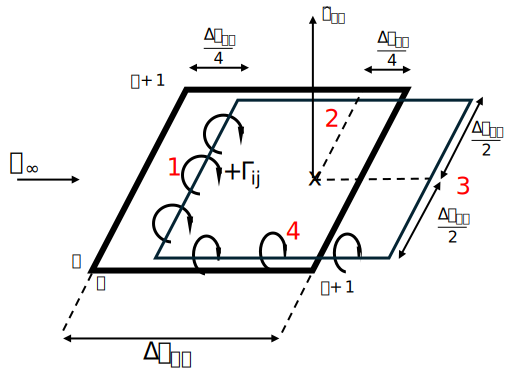
\includegraphics[width=0.8\textwidth]{Quadrilateral vortex ring element.png}
  \caption{Vortex Ring Element}
  \label{fig:VortexRingElement}
\end{figure}



The numbers 1 through 4 on \autoref{fig:VortexRingElement} Vortex Ring Element represent the
four finite straight vortex segments that make up the element. The
induced velocity of the element can be calculated using equation
\eqref{eq:V12} on each segment separately. For an arbitrary point in space
$P(x,y,z)$ the induced velocity is:

\begin{equation}
{\vec{V}}_{P} = {\vec{V}}_{1} + {\vec{V}}_{2} + {\vec{V}}_{3} + {\vec{V}}_{4}
\end{equation}

Where:

\begin{equation}
    \label{eq:Vi}
{\vec{V}}_{i} = \frac{\Gamma}{4\pi}\ \frac{{\vec{r}}_{i,1} \times {\vec{r}}_{i,2}}{\left| {\vec{r}}_{i,1} \times {\vec{r}}_{i,2} \right|}({\vec{r}}_{i,1} - {\vec{r}}_{i,2}) \cdot \left( \frac{{\vec{r}}_{i,1}}{\left| {\vec{r}}_{i,1} \right|} - \frac{{\vec{r}}_{i,2}}{\left| {\vec{r}}_{i,2} \right|} \right)
\end{equation}

These elements are sorted in a two-dimensional grid to cover the lifting
surface shape. To satisfy the trailing edge condition (Kutta condition)
the trailing vortex of the last panel row must be cancelled. Therefore
the last row of panels as well as all the wake panels have the same
circulation $\Gamma$.

\begin{figure}[H]
    \centering
    \includegraphics[width=\textwidth]{vortex ring model.png}
    \caption{Vortex ring elements in a grid \cite{katz2001}}
\end{figure}


The influence coefficient $\alpha_{ij}$ is essentially the induced
velocity of the i-th vortex ring element with unitary circulation at the
j-th collocation point. The influence coefficients can easily be
calculated using equation \eqref{eq:Vi}. Iterating over all panels and all
collocation points results in a matrix

\begin{equation}
A = \begin{bmatrix}
a_{11} & a_{12} & \cdots & a_{1m} \\
a_{21} & a_{22} & \cdots & a_{2m} \\
 \vdots & \vdots & \ddots & \vdots \\
a_{m1} & a_{m2} & \cdots & a_{mm}
\end{bmatrix}
\end{equation}

\begin{figure}[H]
  \centering
  \includegraphics[width=\textwidth]{2D ARRAY OF PANELS.png}
  \caption{Array of wing and wake panel corner points (dots) and of collocation points( $\times$ symbols) \cite{katz2001}}
\end{figure}

For the sake of completeness, the linear set of equations that has to be
solved in order to calculate the circulation intensity of each element
given a certain angle of attack for each panel is:

\begin{equation}
\begin{bmatrix}
a_{11} & a_{12} & \cdots & a_{1m} \\
a_{21} & a_{22} & \cdots & a_{2m} \\
 \vdots & \vdots & \ddots & \vdots \\
a_{m1} & a_{m2} & \cdots & a_{mm}
\end{bmatrix}\begin{bmatrix}
\Gamma_{1} \\
\Gamma_{2} \\
 \vdots \\
\Gamma_{m}
\end{bmatrix} = \begin{bmatrix}
 - {\vec{Q}}_{\infty} \cdot {\hat{n}}_{1} \\
 - {\vec{Q}}_{\infty} \cdot {\hat{n}}_{2} \\
 \vdots \\
 - {\vec{Q}}_{\infty} \cdot {\hat{n}}_{m}
\end{bmatrix}
\end{equation}


The downwash induced at each vortex ring element can be calculated by another set of linear equations

\begin{equation}
\begin{bmatrix}
{w_{ind}}_{1} \\
{w_{ind}}_{2} \\
 \vdots \\
{w_{ind}}_{m}
\end{bmatrix} = \begin{bmatrix}
b_{11} & b_{12} & \cdots & b_{1m} \\
b_{21} & b_{22} & \cdots & b_{2m} \\
 \vdots & \vdots & \ddots & \vdots \\
b_{m1} & b_{m2} & \cdots & b_{mm}
\end{bmatrix}\begin{bmatrix}
\Gamma_{1} \\
\Gamma_{2} \\
 \vdots \\
\Gamma_{m}
\end{bmatrix}
\end{equation}


The lift and drag can then be calculated by using the relationships:

\begin{multline}
    L = \sum_{i = 1}^{M} \sum_{j = 1}^{N} \Delta L_{ij}, \\
    \text{where} \quad \Delta L_{ij} = \begin{cases}
      \rho Q_{\infty} \left( \Gamma_{i,j} - \Gamma_{i - 1,j} \right) \Delta y_{ij}, & \text{for } i > 1 \\
      \rho Q_{\infty} \Gamma_{ij} \Delta y_{ij}, & \text{for } i = 1
    \end{cases}
  \end{multline}

\begin{multline}
D = \sum_{i = 1}^{M} \sum_{j = 1}^{N} \Delta D_{ij}, \\
\text{where} \quad \Delta D_{ij} = \begin{cases}
    \rho w_{\text{ind}_{i,j}} \left( \Gamma_{i,j} - \Gamma_{i - 1,j} \right) \Delta y_{ij}, & \text{for } i > 1 \\
    \rho w_{\text{ind}_{i,j}} \Gamma_{ij} \Delta y_{ij}, & \text{for } i = 1
\end{cases}
\end{multline}


\section{Flutter Analysis Equations}\label{flutter-analysis-equations}

The general form of the aeroelastic equation of motion is \cite{AeroelasticityWright}

\begin{equation}
    \lbrack A\rbrack\ddot{q} + \left( \rho V\lbrack B\rbrack + D \right)\dot{q} + \left( \rho V^{2}\lbrack C\rbrack + \lbrack E\rbrack \right)q = \lbrack 0\rbrack  
\end{equation}



Where:

\begin{itemize}
\item
  $[A]$, $[C]$, and $[E]$, are the structural matrices corresponding to the $[M]$, $[C]$ and
  $[K]$ matrices which is the classical notation used in structural analysis
\item
  $[B]$ and $[C]$ are the aerodynamic matrices which depend on the Mach number
  and the reduced frequency. The way these matrices are computed can
  vary depending on the aerodynamic theory used.
\item
  $q$ are the generalized modal coordinates.
\end{itemize}


\subsection{Interconnection of the Structure with Aerodynamics -- Infinite Plate splines}\label{interconnection-of-the-structure-with-aerodynamics-infinite-plate-splines}

The structural and aerodynamic degrees of freedom are connected by
interpolation. This allows the independent selection of grid points
(nodes) of the structural and aerodynamic matrices thus decoupling the
two discretizations of geometry. This interpolation method is called
splining. The Infinite plate spline which is used here is based on the
structural deformation of a theoretically infinite plate subject to
point loads at given points. The splines are used for two distinct
purposed: as a force interpolator to compute the structurally equivalent
force distribution on the structure given a force distribution on the
aerodynamic mesh and as a displacement interpolator to compute a set of
aerodynamic displacements given as a set of structural displacements.
Mathematically this means that:

\begin{equation}
F_{s} = \left\lbrack G_{s \rightarrow a} \right\rbrack F_{a},\ \ U_{a} = {\lbrack G}_{a \rightarrow s}\rbrack U_{s}
\end{equation}


Where:

\begin{itemize}
\item
  $F_{s}$ and $F_{a}$ are the structural and aerodynamic force
  vectors
\item
  $U_{a}$ and $U_{s}$ are the aerodynamic and structural
  displacement vectors
\item
  $G_{s \rightarrow a}$ and $G_{a \rightarrow s}$ are the spline
  matrices connecting the structural to aerodynamic and vice versa. It
  has been proven by the virtual work principle that the two spline
  matrices are the transform of one another i.e.
  $\left\lbrack G_{s \rightarrow a} \right\rbrack = {{\lbrack G}_{a \rightarrow s}\rbrack}^{T}$
\end{itemize}

\begin{figure}[H]
  \centering
  \includegraphics[width=0.9\textwidth]{surface spline.png}
  \caption{Surface Spline coordinate system \cite{msc2021}}
\end{figure}

The Infinite plate spline and all other surface splines are used to find
a surface in the form $w(x,y)$ for all points $(x,y)$ when w is
known at a discrete set of points
$w_{i} = w\left( x_{i},y_{i} \right)$.

The Infinite plate spline mimics the behavior of an infinite plate under
point load. The deflection of such a plate due to a single concentrated
load at $\left( x_{i} = 0,\ y_{i} = 0 \right)$ is called the
fundamental solution. The governing equation is:



\begin{equation}
D\nabla^{4}(w) = D\frac{1}{r}\frac{d}{dr}\left\{ r\frac{d}{dr}\left\lbrack \frac{1}{r}\frac{d}{dr}\left( r\frac{dw}{dr} \right) \right\rbrack \right\} = q
\label{eq:splineequation}
\end{equation}



The general solution to the homogeneous form of \autoref{eq:splineequation} is:

\begin{equation}
w = C_{1} + C_{1}r^{2} + C_{2}\ln(r) + C_{3}r^{2}\ln(r)
\end{equation}

Setting $C_{2} = \ 0\ $to keep the solution finite at $r = 0$ then
integrating from $r = 0$ to $r = \epsilon\ (small\ number)$ leads to
$C_{3} = \frac{P}{8\pi D}$. Thus, the fundamental solution for a
concentrated load is:

\begin{equation}
w = A + Br^{2} + \frac{P}{16\pi D}r^{2}\ln\left( r^{2} \right)
\end{equation}


The fundamental solution can be superimposed to solve the entire plate
problem:

\begin{equation}
w(x,y) = \alpha_{0} + \alpha_{1}x + \alpha_{2}y + \sum_{i = 1}^{N}{K_{i}(x,y)P_{i}}
\end{equation}


Where:

\begin{itemize}
\item
  $K_{i}(x,y) = \frac{1}{16\pi D}r_{i}^{2}\ln\left( r_{i}^{2} \right)$
\item
  $r_{i}^{2} = \left( x - x_{i} \right)^{2} + \left( y - y_{i} \right)^{2}$
\item
  $P_{i}$ concentrated load at $\left( x_{i},y_{i} \right)$
\end{itemize}

The $N+3$ unknowns of are determined from the $N+3$ equations

\begin{equation}
\sum_{}^{}{Pi} = 0
\end{equation}

\begin{equation}
  \sum_{}^{}{x_{i}P_{i}} = 0
\end{equation}

\begin{equation}
  \sum_{}^{}{y_{i}P_{i}} = 0
\end{equation}

\begin{equation}
  w_{j} = a_{0} + a_{1}x_{j} + a_{2}y_{2} + \sum_{i = 1}^{N}K_{ij}P_{i},\ \ (\ j = 1,\ldots,\ N)  
\end{equation}

Where $K_{ij} = K_{i}\left( x_{j},y_{j} \right)$ and
$K_{ij} = K_{ji},\ \ K_{ij} = 0\ when\ i = j$

These $N+3$ equations can be expressed into a matrix form:

\begin{equation}
\begin{bmatrix}
  \begin{array}{c}
    0 \\
    0 \\
    0 \\
    \hline
    w_{1} \\
    w_{2} \\
     \vdots \\
    w_{N}        
  \end{array}
\end{bmatrix} = \begin{bmatrix}
\begin{array}{cccccc}
  0 & 0 & 0 & 1 & \cdots & 1 \\
0 & 0 & 0 & x_{1} & \cdots & x_{N} \\
0 & 0 & 0 & y_{1} & \cdots & y_{N} \\
\hline 
1 & x_{1} & y_{1} & 0 & \cdots & K_{1N} \\
1 & x_{2} & y_{2} & K_{21} & \cdots & K_{2N} \\
 \vdots & \vdots & \vdots & \vdots & \cdots & \vdots \\
1 & x_{N} & y_{N} & K_{N1} & \cdots & 0
\end{array}
\end{bmatrix}
\begin{bmatrix}
  \begin{array}{c}
    a_{0} \\
    a_{1} \\
    a_{2} \\
    \hline
    P_{1} \\
    P_{2} \\
     \vdots \\
    P_{N}
        
  \end{array}
\end{bmatrix} = \lbrack C\rbrack\lbrack P\rbrack
\end{equation}



Now that the $a_{i}$ and $P_{i}$ any quantity can be interpolated at
any point in the $(x,y)$ plane using the following matrix equation:

\begin{equation}
\left\{ w \right\} = \begin{bmatrix}
1 & x_{1} & y_{1} & K_{1,1} & K_{1,2} & \cdots & K_{1,n} \\
1 & x_{2} & y_{2} & K_{2,1} & K_{2,2} & \cdots & K_{2.m} \\
 \vdots & \vdots & \vdots & \vdots & \vdots & \cdots & \vdots \\
1 & x_{n} & y_{n} & K_{n,1}\  & K_{n,2} & \cdots & K_{n,n}\ 
\end{bmatrix} \cdot \lbrack C\rbrack^{- 1}\begin{bmatrix}
0 \\
0 \\
0 \\
w_{1} \\
w_{2} \\
 \vdots \\
w_{N}
\end{bmatrix}
\end{equation}

\subsection{The PK Method of Flutter Solution}
\label{the-pk-method-of-flutter-solution}

The fundamental equation for modal flutter analysis by the PK method is \cite{msc2021}:

\begin{equation}
\left\lbrack M_{hh}p^{2} + \left( B_{hh} - \frac{1}{4}\rho cV\frac{Q_{hh}^{I}}{k} \right)p + \left( K_{hh} - \frac{1}{2}\rho V^{2}Q_{hh}^{R} \right)\  \right\rbrack \cdot \left\{ u_{h} \right\} = \underline{0}
\end{equation}


Where:

\begin{itemize}
\item
  $M_{hh} =$ modal mass matrix, usually diagonal
\item
  $B_{hh} =$ modal damping matrix
\item
  $K_{hh} =$ modal stiffness matrix, usually diagonal, may be complex
  if actual damping is used
\item
  $Q_{hh}(M,k) =$ aerodynamic force matrix which is a function of mach
  number and reduced frequency $k = \frac{\omega\overline{c}}{2V}$
\item
  $Q_{hh}^{R},\ Q_{hh}^{I}$ are the real and imaginary parts of the
  aerodynamic force matrix $Q_{hh}$ also called aerodynamic stiffness
  and aerodynamic damping matrices respectively
\item
  $k = \frac{\omega\overline{c}}{2V}$ reduced frequency
\item
  $M =$ Mach number
\item
  $V = \ $Velocity
\item
  $\rho =$ fluid density
\item
  $\left\{ u_{h} \right\} =$ modal amplitude vector (modal
  participation vector)
\item
  $p = \omega(\gamma \pm i)$ eigenvalue
\end{itemize}


The equation is rewritten in the state-space form with order reduction

\begin{equation}
    \label{eq:PKss}
\lbrack A - pI\rbrack\left\{ {\overline{u}}_{h} \right\} = 0
\end{equation}

Where:

\begin{equation}
\lbrack A\rbrack = - \begin{bmatrix}
\mathbf{\lbrack 0\rbrack} & \mathbf{\lbrack I\rbrack} \\
 - M_{hh}^{- 1}\left( K_{hh} - \frac{1}{2}\rho V^{2}Q_{hh}^{R} \right) & - M_{hh}^{- 1}\left( B_{hh} - \frac{1}{4}\rho cV\frac{Q_{hh}^{I}}{k} \right)
\end{bmatrix}
\end{equation}

\begin{equation}
  {\overline{u}}_{h} = \begin{bmatrix}
    u_{h} \\
    {\dot{u}}_{h}
    \end{bmatrix}\  
\end{equation}


The basic algorithm for the pk method involves the following steps:

\begin{enumerate}
\def\labelenumi{\arabic{enumi}.}
\item
  Make an initial guess of the frequency for the mode
\item
  Calculate the corresponding reduced frequency $k$ and airspeed $V$
\item
  Determine (by interpolation) the aerodynamic stiffness and damping
  matrices $Q_{hh}^{R},\ Q_{hh}^{I}$
\item
  Determine the frequencies for the system at this flight condition
  using Equation \eqref{eq:PKss}
\item
  Take the frequency solution that was closest to the initial guess and
  repeat steps 1-5 until the frequency converges
\item
  Store the final modal frequency and modal damping
\item
  Consider the next mode of interest using the same procedure until all
  modes of interest have been investigated
\end{enumerate}


\section{Optimization techniques }
\label{optimization-techniques}

\subsection{Brent's -- Dekker Line search method }
\label{brents-dekker-line-search-method}

This algorithm aims to find the minimum of a function of one
variable without using its derivatives. This algorithm is commonly used
when finding the minimum of a function $g\left( \mathbf{x} \right)$ of
several variables \cite{brent1973}. To this end the following function often needs to be
minimized

\begin{equation}
    \label{eq:minfun}
\gamma(\lambda) = f(\mathbf{x}_{0} + \lambda\mathbf{s})
\end{equation}

where $\mathbf{x}_{0}$ and $\mathbf{s}$ are fixed and $\lambda$ is
a scalar variable. This problem essentially describes a one-dimensional
search beginning form $\mathbf{x}_{0}$ in the direction of
$\mathbf{s}$.

The algorithm finds an approximation to the minimum of a function $f$
defined on the interval $\lbrack a,\ b\rbrack$. There are six
significant points $a,b,u,v,w\ and\ x$ not all distinct. These points
are initialized as follows:

\begin{equation}
    \label{eq:brentspoints}
v = w = x = a + \left( \frac{3 - \sqrt{5}}{2} \right)(b - a)
\end{equation}

The number $\left( \frac{3 - \sqrt{5}}{2} \right)$ comes from the
golden section search algorithm and is somewhat arbitrary. The points
defined in \eqref{eq:brentspoints} serve a specific purpose:


\begin{itemize}
\item
  Points $a$ and $b$ define the interval within which a local
  minimum lies
\item
  $x$: of all the points at which $f$ has been evaluated, $x$ is
  the one with the least value of $f$
\item
  $w$ is the point with the next lowest value of $f$
\item
  $v$ is the previous value of $w$
\item
  $u$ is the last point at which f has been evaluated
\end{itemize}

\begin{figure}
  \centering
  \includegraphics[width=\textwidth]{brents_six_points.png}
  \caption{A possible configuration of points \cite{brent1973} }
\end{figure}

A typical iteration of the algorithm evolves as follows:


\begin{enumerate}
\def\labelenumi{\arabic{enumi}.}
\item
  Let $m = 1\text{/}2(a + b)$ be the midpoint of the interval

  \begin{enumerate}
  \def\labelenumii{\alph{enumii}.}
  \item
    If $|x - m| \leq 2 \cdot tol - \frac{1}{2}(b - a)\ $then the
    algorithm terminates with x as the minimum
  \item
    Otherwise, the numbers $p$ and $q$ are calculated such that
    $x + p/q$ is the minimum of the parabola passing through
    points\\
    $\left( v,f(v) \right),\ \ \left( w,f(w) \right),\ \ \left( x,f(x) \right)$
  \end{enumerate}
\item
  Let $e$ be the value of $p/q$

  \begin{enumerate}
  \def\labelenumii{\alph{enumii}.}
  \item
    If $|e| \leq tol$,
    $q = 0$,$x + p\text{/}q \notin \lbrack a,b\rbrack$ or
    $\left| p\text{/}q \right| \geq 1/2|e|$ then the golden ration
    step is performed:
  



\begin{equation}
  u =
  \begin{cases} 
  \frac{\sqrt{5} - 1}{2}x + \frac{3 - \sqrt{5}}{2}a, & \text{if } x \geq m \\ 
  \frac{\sqrt{5} - 1}{2}x + \frac{3 - \sqrt{5}}{2}b, & \text{if } x < m
  \end{cases}
\end{equation}

\item
  Otherwise $u = x + p\text{/}q$ (the
  distances$|u - x|,\ \ u - a,\ \ b - u\ $must be at least $tol$)
\end{enumerate}
\end{enumerate}


\begin{enumerate}
\def\labelenumi{\arabic{enumi}.}
\setcounter{enumi}{2}
\item
  $f$ is evaluated at the new point $u$ the points
  $a,b,v,w\ and\ x$ are updated and the cucle repeats
\end{enumerate}

The algorithm typically terminates when $x = b - tol$ or
$x = a + tol$ after a parabolic interpolation has been performed where
the condition that $|u - x| \geq tol$ has been enforced. The next
parabolic interpolation point lies close to x and b so u is forced to be
$x - tol$.

\begin{figure}[H]
    \centering
    \includegraphics[width=\textwidth]{brents algorithm termination configuration.png}
    \caption{typical terminal configuration of important points \cite{brent1973}}
\end{figure}

\subsection{Powell's Method}
\label{powells-method}

Powell's method is a modified cyclic coordinate search. Both methods aim
to minimize a multivariate function without using any of its
derivatives. That's why they are called zero-order methods.

The Cyclic coordinate search method is in essence a series of
line-search optimizations performed cyclically over all inputs of the
function. The search starts from an initial $x^{(0)}$ and optimizes
the first input:

\begin{equation}
\mathbf{x}^{(1)} = \arg_{x_{1}}{\min{f\left( x_{1},x_{2}^{(0)},\ldots,x_{n}^{(0)} \right)}}
\end{equation}

Having solved this, it optimizes the next coordinate:

\begin{equation}
\mathbf{x}^{(2)} = \arg_{x_{2}}{\min{f\left( x_{1}^{(1)},x_{2},\ldots,x_{n}^{(1)} \right)}}
\end{equation}

This can also be expressed with the help of equation \eqref{eq:minfun} if
$\mathbf{s}$ is the i\textsuperscript{th} basis vector for
$i = 1,\ldots,n$

Any line search algorithm can be used but Brent's Algorithm has seen
wide usage in optimization libraries including SciPy's implementation of
the Powell method.

\begin{figure}[H]
    \centering
    \includegraphics[width=0.5\textwidth]{cyclic coordinate search.png}
    \caption{Cyclic coordinate search \cite{kochenderfer2019}}
    \label{fig:CCsearch}
\end{figure}

As can be seen in \autoref{fig:CCsearch} a weakness of this method is the slow
traversal of diagonal valleys where repeated small steps are taken in
every direction. M.J.D. Powell's idea was to expand the cyclic
coordinate search method so that it can search in directions that are
not orthogonal to each other and are also not the basis vectors. In
order to achieve this new capability, Powell's algorithm maintains a list
of search directions
$\left\lbrack \mathbf{u}^{(0)},\ldots\mathbf{u}^{(n)} \right\rbrack$
which are initially the coordinate basis vectors
$\mathbf{u}^{(i)}=\mathbf{e}^{\left( \mathbf{i} \right)}$ for
all $i$.

Starting at $\mathbf{x}^{(0)}$ Powell's method conducts a line search
as before for each search direction in succession:


\begin{equation}
\mathbf{x}^{(i + 1)} \leftarrow linesearch\left( f,\mathbf{x}^{(i)}\mathbf{,}\mathbf{u}^{(i)} \right)\mathbf{\ }for\ i\ in\ \lbrack 0,\ldots,n\rbrack
\end{equation}

Next the all the search directions are shifted down by one index
dropping the oldest search direction,$\mathbf{u}^{(0)}\ $

\begin{equation}
\mathbf{u}^{(i)} \leftarrow \mathbf{u}^{(i + 1)}\ for\ i\ in\ \lbrack 0,\ldots,n - 1\rbrack
\end{equation}

The last search direction is replaced with the direction from
$\mathbf{x}^{(0)}$ to $\mathbf{x}^{(n + 1)}$, which is the overall
direction of progress over the last n line searches:

\begin{equation}
\mathbf{u}^{(n)} \leftarrow \mathbf{x}^{(n + 1)} - \mathbf{x}^{(0)}
\end{equation}

This process is repeated until convergence.
\begin{figure}[H]
    \centering
    \includegraphics[width=0.5\textwidth]{powells method.png}
    \caption{Powell's method \cite{kochenderfer2019}}
    \label{fig:Powell}

\end{figure}

As can be seen in \autoref{fig:Powell} Powell's method begins the same as cyclic
coordinate search but gradually learns conjugate direction.


\subsection{Genetic Algorithm}
\label{genetic-algorithm}

Genetic algorithms mimic the logic behind Darwinian evolution, where the
fitter individuals are more likely to pass on their genes to the next
generation. The chromosomes of each individual define a single design
point. At each generation the chromosomes of the fitter individuals are
passed on to the next generation after undergoing the genetic operation
of \emph{crossover} and \emph{mutation}

Chromosomes are often represented by a binary array but in this case an
array of real values describes the design space better.

\subsubsection{Initialization}

The Genetic Algorithm begins by initializing a population with random
chromosomes

\subsubsection{Parent Selection}

The selection process is the process of choosing which chromosomes will
be selected to create offsprings for the next generation after being
subjected to the crossover and mutation genetic processes. There are
many methods of selecting which individuals get to mate and combine
their genes, some of the most popular include:

\begin{itemize}
\item
  Roulette Wheel selection: Where each individual is assigned an area of
  an imaginary roulette proportional to their fitness. Then the roulette
  is spun until the desired number of parents is reached. This method is
  simple and effective in most cases. It can become overwhelmed by
  individuals who are much fitter than the rest of the population
\item
  Tournament selection: A subset of individuals is selected at random
  and then the best from this subject is selected as a parent. The
  process is repeated until the desired number of parents is reached
\item
  Steady state Selection: A steady portion of the population is replaced
  at each generation. Only the weakest individuals are replaced by
  offsprings, this method insures that the fittest individual is
  maintained most of the time. A disadvantage of this method is that it
  is slow to adapt as only a small portion of the population is replaced
  at every generation
\end{itemize}

\subsubsection{Crossover}

Crossover is the way the chromosomes of the parents are combined to
create an offspring. There are several crossover schemes. The most
commonly used are :
\begin{samepage}
\begin{itemize}
\item
  Single point crossover

In this scheme the first portion of parent A forms the first portion for the child chromosome and the latter portion of parent B's chromosome
forms the latter part of the child chromosome.

\begin{figure}[H]
    \centering
    \includegraphics[width=\textwidth]{single point crossover.png}
    \caption{Single Point Crossover \cite{kochenderfer2019}}

\end{figure}


\item
  Two-point crossover


Same as before but a second crossover point is added.

\begin{figure}[H]
    \centering
    \includegraphics[width=\textwidth]{two point crossover.png}
    \caption{Two-point Crossover \cite{kochenderfer2019}}

\end{figure}

\item
  Uniform crossover


In this scheme every chromosome has a 50\% chance of coming from parent
A or parent B.
\begin{figure}[H]
    \centering
    \includegraphics[width=\textwidth]{uniform crossover.png}
    \caption{Uniform Crossover \cite{kochenderfer2019}}

\end{figure}
\end{itemize}
\end{samepage}

\subsubsection{Mutation}

Mutation is a necessary step of the genetic algorithm since it allows new traits to develop which were not present in the initial population. In essence a random value is added to a random chromosome of a randomly selected offspring. The chance of a mutation occurring to an individual is called the \emph{mutation rate}

\subsubsection{Elitism}

Elitism is a strategy that ensures that a fixed number of the most fit
individuals survive to the next generation

Genetic algorithms have a very wide spectrum of application and are very adaptable to many problems. But there is a catch. All those parameters and strategies affect the results greatly and there exists no standard method of selecting every parameter. So, it is the responsibility of the researcher to understand the problem at hand and through experimentation and model hyperparameter tuning techniques determine a
good enough set of parameters.

\subsection{Neural Networks}
\label{neural-networks}

\subsubsection{What are Artificial Neural Networks (ANN's)}

An artificial neural network is a computational model which draws inspiration from the way a biological brain works. The basic structure of an ANN consists of interconnected nodes (or neurons) organized in layers.

The base unit of this structure is a neuron. A neuron has a very simple structure. It accepts an arbitrary number of inputs along with a bias and only has one output. The output can be binary or scalar. Within the neuron a summation is performed using the weight of each input and the bias. The result of each summation is further processed through an ``activation function'' and the output is reached. The activation function allows for nonlinear behavior of the neural networks. It can be
any function, but some functions have prevailed.

\begin{figure}[H]
    \centering
    \includesvg[width=\textwidth]{Neuron.svg}
    \caption{The Structure of a Neuron}

\end{figure}


The basic architecture of a neural network consists of:

\begin{enumerate}
\def\labelenumi{\arabic{enumi}.}
\item
  An input layer which is responsible for receiving the initial data.
  Each neuron in the input layer depicts a specific feature or attribute
  of the input data
\item
  Hidden layers, which are intermediate layers between the input and
  output layers which are responsible for complex feature recognition.
\item
  The weights and biases which are to be used in the neural network, and
  which are the parameters to be trained in order for the neural network
  to make meaningful predictions.
\item
  An output layer which generates the final predictions. The output can
  be binary for classification problems or scalar for regression
  problems.
\end{enumerate}

\begin{figure}[H]
    \centering
    \includesvg[width=\textwidth]{Neural Network.svg}
    \caption{Structure of a Neural Network \cite{takyar2025}}

\end{figure}

The number of Hidden layers in a neural network can vary. Neural
networks which do not have any hidden layers are called ``shallow'', on
the other hand Neural Networks with hidden layers are called Deep Neural
Networks.

\subsubsection{Artificial Neural Network Training}

As stated previously, for a neural network to be useful it has to be trained. Training involves gathering data similar to the ones that the NN is supposed to predict and then performing an optimization of the weights and biases within this network to minimize some loss function. A loss function is a measure of the amount of error. There are many loss functions commonly used for Neural networks, but when a Neural network
is trained on a regression problem the loss function is usually one of the following:

\begin{enumerate}
\def\labelenumi{\arabic{enumi}.}
\item
  Mean Squared Error (MSE)
\end{enumerate}

\begin{equation}
MSE = \frac{1}{N}\sum_{i = 1}^{N}\left( y_{i} - \hat{y} \right)^{2}
\end{equation}

\begin{enumerate}
\def\labelenumi{\arabic{enumi}.}
\setcounter{enumi}{1}
\item
  Root Mean Squared Error
\end{enumerate}

\begin{equation}
RMSE = \ \sqrt{MSE} = \sqrt{\frac{1}{N}\sum_{i = 1}^{N}\left( y_{i} - \hat{y} \right)^{2}}
\end{equation}

\begin{enumerate}
\def\labelenumi{\arabic{enumi}.}
\setcounter{enumi}{2}
\item
  Mean Average Error (MAE)
\end{enumerate}

\begin{equation}
MAE = \frac{1}{N}\sum_{i = 1}^{N}{|y_{i} - \hat{y}|}
\label{eq:MAE}
\end{equation}

Where: $\hat{y}\ is\ the\ predicted\ value\ of\ y$

Minimizing any of these functions on test data that the network hasn't
seen before is the goal of training.

To achieve this goal first the available data which contain both the input and the wanted output, are randomly split between training data (those that will be used for the adjustment of weights and biases) and test data (those which will be used to judge the performance of the neural network). Then through a process called backpropagation (the exact explanation of which is beyond the scope of this thesis) on batches of the training data the weights are updated in such a way so as to reduce the value of the loss function for this particular set of data points. Once all the batches of data have been run through the network and the weights have been adjusted accordingly, we say that the network has completed one pass through the training data This procedure estimates the negative gradient of the loss function and so the network works its way down the slope of the loss function. The number of times this procedure is repeated is called epochs. The number of epochs should be such that an optimum solution is reached without overfitting the network to the test data.

\subsubsection{Hyperparameter Tuning}

As we have seen, in order to define a neural network many parameters have to be chosen in advance. Those parameters include the number of hidden layers, the number of neurons in each layer along with the activation function of each layer to name a few. The best set of parameters is not known a priori and there is no method of selecting the
optimal set.

The process of optimization of a model's hyperparameters is called \emph{hyperparameter tuning}. There are many optimization algorithms that achieve this. One of the more interesting ones and the one that will be employed for this application is the HyperBand algorithm \cite{li2018hyperbandnovelbanditbasedapproach}. The algorithm is an improvement of the Successive Halving
algorithm.

The Idea behind the Successive halving algorithm is quite simple. It uniformly allocates a budget of resources (computational time) to a set of hyperparameters evaluates the performance of each test, reject the bottom 50\% and repeat until one configuration remains. The problem with this algorithm is that it is not known whether testing a larger number of configurations with limited budget each or a smaller number of configurations with more budget will result in a better outcome.

This is the problem that the HyperBand algorithm was made to tackle. It does this by performing a grid search over feasible values of $n$ and $r$, where $n$ is the number of configurations to be tested and $r$ is the minimum resource that is allocated to all configurations before they are allowed to be discarded.